\section{A cosmological acceleration scale: prediction and tension}
\label{sec:redshift}

The model predicts an acceleration scale proportional to the cosmic
expansion rate, with its coefficient fixed by equation~\eqref{eq:eps}.
Using the background specified for this comparison gives
\begin{equation}
\frac{a_0(z)}{10^{-10}\,\mathrm{m\,s^{-2}}}
=1.23072924\sqrt{0.315(1+z)^3+0.685}.
\label{eq:aznumeric}
\end{equation}
Its linear projection over $0.33\le z\le1.44$ is
\begin{equation}
\frac{a_0^{\rm line}(z)}{10^{-10}\,\mathrm{m\,s^{-2}}}
=1.002784+1.225645z.
\label{eq:projection}
\end{equation}
The published MOND-based kinematic analysis in Appendix E of
Ciocan et al. gives an intercept $1.03\pm0.05$ and slope
$1.20\pm0.10$ in these units. The main-text dark-halo decomposition gives a
larger slope, about $1.59$. These are distinct inferences from the
kinematic analysis and must be compared separately. \cite{ciocan}

\subsection{What is measured}

For a nearly circular stellar or gas orbit, the inferred centripetal
acceleration is
\begin{equation}
g_{\rm obs}(r)=\frac{v_c^2(r)}{r}.
\end{equation}
A baryonic model supplies the acceleration $g_b$ generated by the observed
stars and gas. The radial acceleration relation, or RAR, describes how
$g_{\rm obs}$ depends on $g_b$. In the galaxy outskirts $g_b$ is small and
the inferred attraction exceeds the Newtonian baryonic value. The
parameter $a_0$ locates the transition.

At intermediate redshift, the rotation field, pressure support, inclination,
gas profile, and stellar mass must be inferred together. Ciocan et al.
explicitly describe the resulting RAR as model dependent. Their Appendix E
refits the kinematics within a MOND framework and then estimates the
redshift dependence. The coefficient comparison here uses that inference;
it does not treat the measurements as a direct model-independent
measurement of the substrate. \cite{ciocan}

\subsection{Why a cosmological acceleration enters}

The Unruh temperature associated with proper acceleration $a$ is
\begin{equation}
k_BT_U=\frac{\hbar a}{2\pi c}.
\end{equation}
For a de Sitter horizon, the corresponding temperature is
\begin{equation}
k_BT_H=\frac{\hbar H}{2\pi}.
\end{equation}
Equating these two scales gives $a=cH$. This relation motivates a
cosmological acceleration scale. Applying a horizon temperature to an
evolving cosmological background requires the chosen horizon-contact
prescription. Neither detector thermality nor dimensional analysis alone
fixes the coefficient of the galactic law. Milgrom related the MOND acceleration scale to the de Sitter
horizon through this temperature comparison, with a different interpolation.
\cite{unruh,gibbons,milgrom1999}

The capacity model supplies that coefficient through the tilt mode of the
transverse frame. The baryonic field is its restoring stiffness and its
inertia lever is $\ell=g\,c/H$, so its frequency is $\omega=\sqrt{g_b/\ell}$.
At the horizon temperature its gap is
$\hbar\omega/k_BT_H=2\pi\omega/H=\sqrt{g_b/a_0}$ with $a_0=\epsilon cH$ and
$\epsilon=g/(4\pi^2)$; for a lever in apparent-horizon radii the factor
$4\pi^2$ is the square of the $2\pi$ in $T_H$.
The construction connects the galaxy's transition scale to an external
cosmological state without adjusting a coefficient for the high-redshift
sample. The tilt-mode identification, its thermalization, and the lever are the
matching inputs described in the theory; the lever coefficient
is the ratio of the register enthalpy to a one-nat oriented record read at
the Unruh temperature of the projected baryonic field, and that reading is
the premise. \source{T1, section 15 and N.8}

The thermal variable is the occupation energy of the transverse response.
The construction assigns no ordinary radiation temperature to an orbiting star.

\subsection{The response law and its limits}

The occupation energy of the tilt mode is
\begin{equation}
E=k_BT_H x,\qquad x=\sqrt{g_b/a_0}.
\label{eq:thermalenergy}
\end{equation}
For a bosonic occupation number $n=0,1,2,\ldots$, the single-mode partition
sum is a geometric series:
\begin{equation}
Z_B=\sum_{n=0}^\infty e^{-nx}=\frac1{1-e^{-x}}.
\end{equation}
The mean occupation follows by differentiation,
\begin{equation}
\langle n\rangle=-\frac{d\ln Z_B}{dx}
=\frac1{e^x-1}=n_B(x).
\end{equation}
Identifying the excess gravitational response with this occupation gives,
in spherical symmetry,
\begin{equation}
g_{\rm obs}=g_b[1+n_B(x)]
=\frac{g_b}{1-e^{-\sqrt{g_b/a_0}}}.
\label{eq:rar}
\end{equation}
In the deep regime $n_B\simeq1/x$ is the equipartition occupation of the
mode, and at high acceleration its Wien suppression returns the Newtonian
field. The Bose sum and spherical response are proved for the tilt-mode
energy and readout. The carrier-action field equations also follow from
compactly supported variations for a smooth interpolating function.
For this response its derivative is singular at zero baryonic field,
so the classical derivation applies on the regular nonzero-field branch;
extension through field zeros requires a weak or regularized treatment.
The square-root energy mapping and horizon contact remain physical
matching conditions. \source{T4}

At $g_b\gg a_0$, the occupation is exponentially small and
$g_{\rm obs}\simeq g_b$. At $g_b\ll a_0$, expansion of the denominator gives
\begin{equation}
g_{\rm obs}=\sqrt{a_0g_b}+\frac12g_b
+O\!\left(\frac{g_b^{3/2}}{\sqrt{a_0}}\right).
\end{equation}
For a pointlike baryonic source, $g_b=GM_b/r^2$, so the leading term implies
\begin{equation}
v_c^4=GM_ba_0.
\end{equation}
This is the baryonic Tully--Fisher scaling. In the proposed contact branch,
its normalization evolves with $H(z)$. The isolated equilibrium response
uses the cosmological contact at the epoch being modeled. A previously
formed, subsequently stripped stock evolves through its own transport history.

A positive finite update can relax radial occupation while preserving
each retained angular-bin mass. Lean verifies this separation, so radial
adjustment need not erase angular memory. In a spherical numerical
example with a chosen $0.5\,$Gyr relaxation time, the force differs from
the evolving target by at most $2.21\%$ today and $12.89\%$ earlier.
Separate live tilted-stock realizations retain stellar tilt for eight
Gyr at a fixed radial target. A common evolution with changing $a_0$,
the required energy exchange, and converged nonspherical forces remains
to be tested. \source{T1, O.3; G7}

\subsection{Why the fitted intercept lies below the local value}

The numerical curve in equation~\eqref{eq:aznumeric} has
$a_0(0)=1.230729\,\aunit$ and $a_0(1)=2.203315\,\aunit$.
The intercept of a line fitted over a positive-redshift interval is a
different quantity from the value of the curved function at zero.

For points $(z_i,f_i)$ with equal weights, minimizing
$\sum_i[f_i-(A+Bz_i)]^2$ gives
\begin{equation}
B=\frac{\sum_i(z_i-\bar z)(f_i-\bar f)}
{\sum_i(z_i-\bar z)^2},\qquad A=\bar f-B\bar z.
\label{eq:linefit}
\end{equation}
Using $z_i=0.33,0.34,\ldots,1.44$ gives equation~\eqref{eq:projection}.
The resulting intercept is $1.003$ and the slope is $1.226$; both are
within the published marginal errors.

The curvature follows analytically. Write
$u=1+z$ and $E=\sqrt{\Omega_m u^3+\Omega_\Lambda}$. Then
\begin{equation}
\frac{d^2E}{dz^2}
=\frac{3\Omega_m u\,[\Omega_m u^3+4\Omega_\Lambda]}{4E^3}>0.
\end{equation}
Across the stated interval, a single straight line averages the increasing
slope and extrapolates below the true value at $z=0$. The lower intercept
therefore has a direct mathematical explanation within the proposed
curve. Its precise size depends on the interval and weights.

\begin{figure}[htbp]
\centering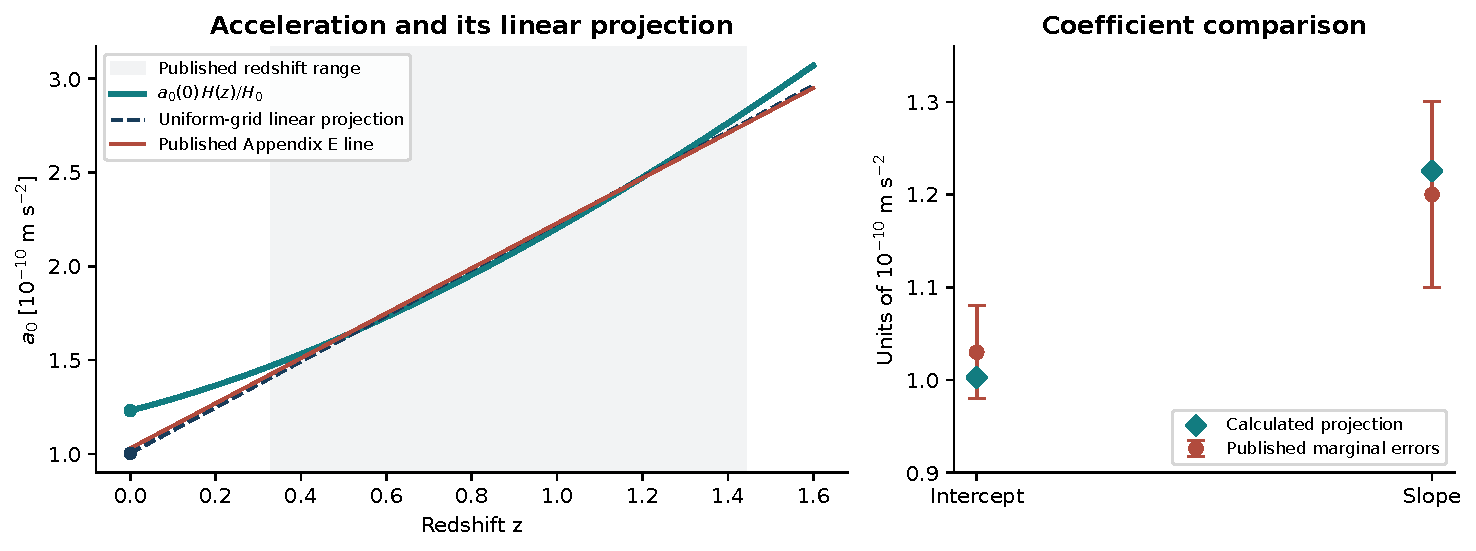
\includegraphics[width=\textwidth]{figures/redshift.pdf}
\caption{The calculated acceleration curve and its linear projection.
The published line summarizes the Appendix E inference. The right panel
shows marginal coefficient errors, with no assumption of independence.
The uniform-grid projection is not a refit to the original galaxy data.}
\end{figure}

The individual coefficient differences are $-0.54$ and $+0.26$ times the
quoted marginal errors. A joint significance requires the fitted
intercept--slope covariance and the survey's effective redshift weighting.
The two agreements are consequences of one curve, not independent
probabilities to multiply.

\subsection{A joint cosmological test}

The prediction fixes the absolute function, including normalization and
curvature. This comparison uses $\Omega_m=0.315$ and
$\Omega_\Lambda=0.685$. A joint test must use the release model's
fitted $H(z)$ in equation~\eqref{eq:a0}, propagate its uncertainty, and
fit the individual galaxies with their correlated baryonic and kinematic
errors. Galaxy formation can also produce an evolving RAR in conventional
halo models, so evolution alone does not distinguish the mechanisms.

\subsection{Catalogue tests and the direction of a relaxation correction}
The common cosmology was propagated to 73 KMOS3D, 21 KGES, and 169 KROSS
objects at three radii. At the KMOS3D outer radius, the log-acceleration
residual slope is $-0.245$ dex per unit redshift with constant $a_0$ and
$-0.313$ with the common $H(z)$ law. The latter has median log-velocity
residual $-0.087$ dex. The reference $z=2.3$ example gives acceleration
boosts about 2.02 versus 1.39 for the compared evolving and fixed scales.
These are catalogue central-value diagnostics with specified baryon force
models; they do not constitute raw-cube likelihoods. The 112-point
reference projection remains distinct from a regression on the actual
79-object MUSE selection. The common cosmology has not removed the
high-redshift residual trend. \source{U1, S01}

Passive relaxation cannot automatically supply a reduction. If
$\dot n=\Gamma(q-n)$ with $\Gamma>0$, $\dot q\le0$, and initially
$n\ge q$, then $n$ remains above the target. At fixed baryons a lag behind
declining $H$ therefore has the wrong sign to suppress an initially
equilibrated response. Underoccupied assembly states require their own
history. Relabeling an unchanged stock leaves its total stress unchanged;
the tested adiabatic cosmological mass loss gives an inferred scale ratio
0.9183 from $z=2.3$, compared with $H_0/H(2.3)=0.2972$.
These constraints identify the contact and preparation history as physical
requirements. \source{D1}

For the selected two-pole quantum response, the noise enhancement
$\mathcal F$ and mean delay $\bar\tau$ obey
$\mathcal F H\bar\tau\ge4$. The illustrative three-percent tracking
condition at occupation argument $x=1$ gives $\mathcal F\gtrsim158$,
requiring about $6.47\times10^4$ independent cells for three-percent
force rms. Actual windows, correlations, and gravitational coupling
remain unspecified, so this is a contact-model constraint.
\source{D1; T1, N.8}

\subsection{Stock selection reaches the response law}
\label{sec:stockselection}
The response law is an equilibrium of the retained stock. The stock
reaches it through a selection with three ingredients:
\begin{itemize}
\item \textbf{Occupation.} The response cell's occupation is the stock
field in baryonic units, $n=g_R/g_b$.
\item \textbf{Free energy.} Its excess free energy is the Bose relative
entropy $D(n\Vert n_*)$. Its weight is fixed by equipartition with the
excess field, $\mathcal N\Theta=g_b^2n_*(1+n_*)/4\pi G$.
\item \textbf{Contacts.} Momentum-conserving stock contacts proceed when
they lower the orbit-averaged free energy, which is the zero-temperature
limit of detailed balance with the horizon bath.
\end{itemize}
A coupling that held the stock at the response density would pass the
stock's kinematic mismatch $d$ to the baryons as a force error $-dJ'(g_b)$,
with $J'\simeq5$ at 100\,kpc. The stock therefore supports itself, and the
selection acts slowly. \source{T1, O.3; G8, G9}

Spherical three-dimensional runs use abundance-matched NFW stock with an
equilibrium Eddington distribution \cite{dutton,moster}, static
spherical-equivalent baryons, and one to three contact proposals per
orbit. They run for 12\,Gyr. Offsets from the response law are rms over
5--200\,kpc, and over 5--100\,kpc for dwarfs:
\begin{center}
\small
\begin{tabularx}{\textwidth}{lccX}
\toprule
Model & no contacts & 8--12\,Gyr & note\\
\midrule
Milky Way, 4 runs & 0.10 & 0.009--0.032 & mismatch falls to the shot-noise level\\
Dwarf, 3 seeds & 0.13 & 0.02--0.04 & 5--10\% above the exact constrained minimum\\
Massive spiral, $6\times10^{12}\Msun$ & 0.03 & 0.007--0.043 & \\
Massive spiral, $2.5\times10^{12}\Msun$ & 0.14 & 0.05 & stock budget binds; still converging\\
Full Bose functional, MW & & 0.019--0.024 & matches its Gaussian limit\\
Full Bose functional, dwarf & & 0.025--0.030 & matches its Gaussian limit\\
\bottomrule
\end{tabularx}
\end{center}
Contacts conserve momentum and angular momentum to roundoff, and the
energy ledger closes to $10^{-3}V_f^2$. The stock gains about $0.15V_f^2$
per unit mass from the work register. The mismatch decreases overall,
with fluctuations at the particle shot-noise level.

\begin{figure}[H]
\centering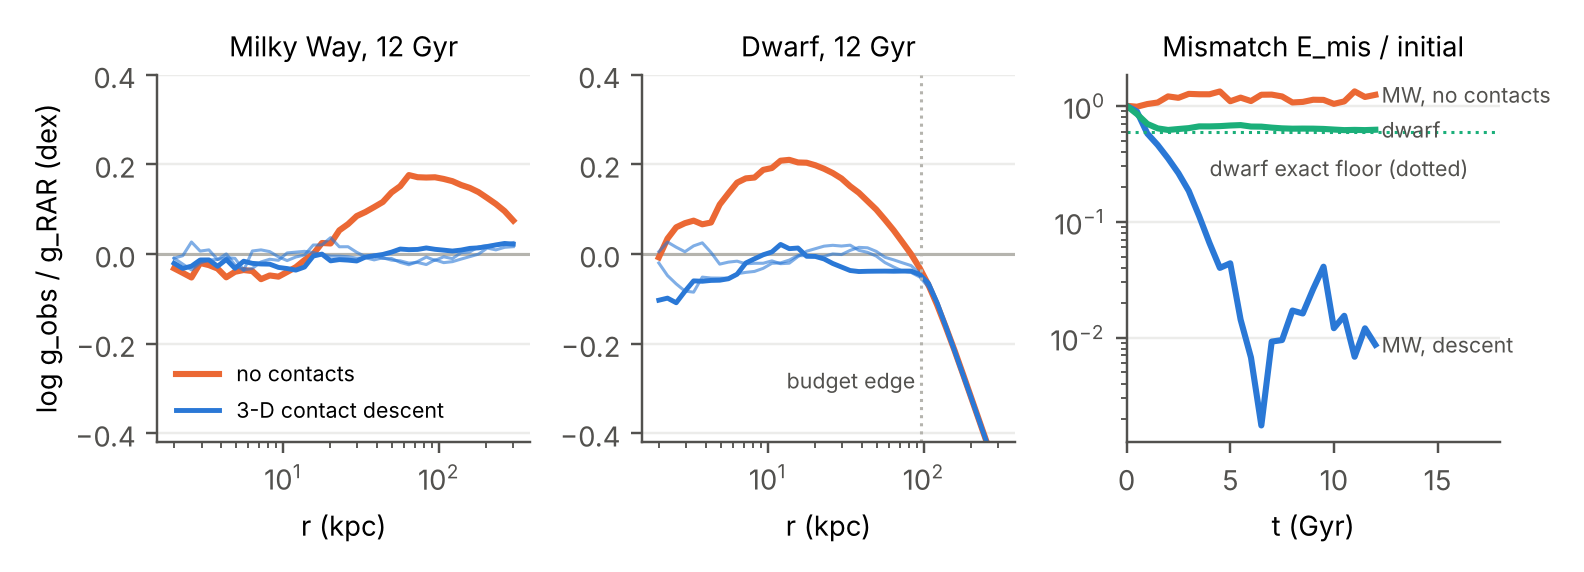
\includegraphics[width=\textwidth]{figures/stock_selection.png}
\caption{Offset from the response law after 12\,Gyr without contacts
(orange) and with contact selection (blue, three runs per model). Right:
the mismatch functional relative to its initial value; the dotted line is
the dwarf's exact constrained minimum.}
\end{figure}

\textbf{The cohort ratio inside galaxies.} Inside radius $r$ the selected
stock-to-baryon ratio equals the occupation $n_*(x)$, which rises
outward. A Milky Way model has about 0.8 inside 10\,kpc, 5.2 at 50\,kpc,
11 at 100\,kpc and 22 at 200\,kpc, up to the budget edge, where the
retained stock is exhausted. A galaxy that has lost most of its ancestral
baryons from the counted region therefore shows a total of about 30 stock
masses per present baryonic mass. The same stock, measured against the
cohort's original baryons, holds the ratio $k_C$.

\textbf{Weak lensing.} An isolated finite stock bounds the excess surface
density by $(1+S)g_{\rm bar}/\pi G$. A signal on the deep response law then
requires $S\ge\tfrac\pi4\sqrt{a_0/g_{\rm bar}}-1$: about 12 at
$4.7\times10^{-13}$, 31 at $7.6\times10^{-14}$ and 275 at
$10^{-15}\,\mathrm{m\,s^{-2}}$. Stocks of about 30 fit the inner KiDS
bins \cite{brouwer21}. The carried stock ends with the support, where
hot gas outweighs the condensed baryons, and the uncarried stock outside
keeps the halo profile. A population forward model of the four isolated
stellar-mass bins of \cite{brouwer21}, with 60 points, full covariance,
the same hot gas and a common environment term, gives $\chi^2=140$ for
the support-limited stock against $133$ for truncated NFW halos when
both fit a halo-mass shift and a concentration factor. Both leave
$3$--$6\sigma$ residuals at $0.5$--$1.5\,$Mpc, where neighbouring
structure contributes. \source{G8, G12}

